% http://www.texample.net/tikz/examples/power-electronics-rectifier/
% Example 4-7, p. 135 of Hart, discontinuous current in full-wave rect
\hspace{-3 cm}
\begin{tikzpicture}
  \begin{scope}[xscale=1.7,yscale=2.8]
    \newcommand{\alphaa}{68 * pi / 180}
    \newcommand{\betaa}{200 * pi / 180}
    \newcommand{\gammaa}{82 * pi / 180}

    \draw[thin, ->] (-3.5, 0) -- (7,0) node[right] {$\omega t$};
    \draw[thin, ->] (0,0) -- (0,1.3) node[left] {$U$};
    
    \foreach \x/\xtext in {{-pi}/{-\pi},{-pi/6}/{-\frac{\pi}{m}}, 0,{pi}/\pi,
      {2*pi}/{2\pi}}
    \draw (\x,0.1) -- (\x,-0.1) node [below] {$\xtext$};

    \draw[thin] (\alphaa, {cos(\alphaa r)}) -- (\alphaa,-0.6) node [below] {};
    \draw[thin, ->] ({pi/6},-0.55) -- (\alphaa,-0.55) node[right] {$\alpha$};
    \draw[thin] ( {pi/6 - 0.05},{-0.55 - 0.05} ) -- ++ (0.1,0.1); 
%    \draw (\betaa,-0.1) -- (\betaa,0.1) node [above] {$\beta$};
    \draw[thin] (\gammaa,-0.40) -- (\gammaa,{cos((\gammaa - pi/3) r)/2 + cos(\gammaa r)/2}) node [above] {};
%    \draw[thin, ->] ({pi/6},-0.35) -- (\gammaa,-0.35) node[right] {$\gamma$};
%    \draw[thin] ( {pi/6 - 0.05},{-0.35 - 0.05} ) -- ++ (0.1,0.1);
    \draw[thin, ->] ({\alphaa-pi/12}, -0.35) -- (\alphaa,-0.35);
    \draw[thin, <-] (\gammaa,-0.35) -- ({\gammaa+pi/12},-0.35) node[below] {$\gamma$};
    
    
     \draw[thin] ({pi/6},{cos((pi/6) r)}) -- ({pi/6},-0.7) node [above] {} ;

    % Vs
    \draw[domain=-3:6.4, help lines, smooth, yellow!97!black]
    plot (\x,{sin((\x + pi/6) r)});

    \draw[domain=-3:6.4, help lines, smooth, green]
    plot (\x,{sin((\x + 60 * pi / 180 + pi/6) r)});

    \draw[domain=-3:6.4, help lines, smooth]
    plot (\x,{sin((\x + 120 * pi / 180 + pi/6) r)});

    \draw[domain=-3:6.4, help lines, smooth]
    plot (\x,{sin((\x + 180 * pi / 180 + pi/6) r)});

    \draw[domain=-3:6.4, help lines, smooth]
    plot (\x,{sin((\x + 240 * pi / 180 + pi/6) r)});

    \draw[domain=-3:6.4, help lines, smooth]
    plot (\x,{sin((\x + 300 * pi / 180 + pi/6) r)});
    
    
    % -Vs

    % Vo and Io
    \foreach \qq [evaluate=\qq as \qqshft using \qq*pi/3] in {-1,...,2}
     {
      \begin{scope}[xshift=\qqshft cm,
          every path/.style={ultra thick, color=red}]
        %Vo
        \draw[domain={pi/6+\gammaa-pi/2}:\alphaa]
        plot (\x,{cos(\x r)})
        -| (\alphaa,{cos((\alphaa - pi/3) r)/2 + cos(\alphaa r)/2})
        [domain=\alphaa:\gammaa]
        plot (\x,{cos((\x - pi/3) r)/2 + cos(\x r)/2 })
        -| (\gammaa, {cos((\gammaa - pi/3) r) })
        ;        
       \end{scope}
     }
     \node[above,color=red] at ({\gammaa + pi/3},1) {$u$};

     % I
     \draw[thin, ->] (-3.5, -1.7) -- (6.4,-1.7) node[right] {$\omega t$};
     \draw[thin, ->] (0,-1.9) -- (0,-1.2) node[left] {$I$};

     \draw[green] ({\gammaa - pi/3},  -1.4) -- (\alphaa, -1.4);
     \draw[green] (\alphaa, -1.4) -- (\gammaa, -1.7);
     \draw[green] (\gammaa, -1.7) -- ({\alphaa + pi/3},-1.7);

     \draw[yellow!97!black] ({\gammaa - pi/3},  -1.7) -- (\alphaa, -1.7);
     \draw[yellow!97!black] (\alphaa, -1.7) -- (\gammaa, -1.4);
     \draw[yellow!97!black] (\gammaa, -1.4) -- ({\alphaa + pi/3},-1.4);

     \draw[thin] (\alphaa,-1.65) -- (\alphaa,-1.9);
     \draw[thin] (\gammaa,-1.65) -- (\gammaa,-1.9);
     \draw[thin, ->] ({\alphaa-pi/12}, -1.8) -- (\alphaa,-1.8);
      \draw[thin, <-] (\gammaa,-1.8) -- ({\gammaa+pi/6},-1.8) node[below] {$\gamma$}; 
  \end{scope}
  \end{tikzpicture}


В $e_k$ содержатся ($E_{2m\phi}$, $L_\phi$, $r_\phi$).
Где $L_\phi$ -- эквивалентная индуктивность приведенная ко вторичной обмотке.
Как определить параметры? Из опыта к.з. Есть измеренные U, I, Z, P.
Из $I^2 R = P$ определим $L_{\textcyrillic{фазы}}$

$X_{\textcyrillic{фазы}}$, $\omega L_{\textcyrillic{фазы}} = 2\pi f L_\phi$.

$U_0$ -- как бы встречная ЭДС.

$U = U_0 + R_D\cdot I$, где $R_D$ -- динамическое сопротивление.

Принимаем допущение $i_d \approx I_d$ -- пренебрегаем пульсациями.
Еще одно допущение $m\ge 2$. Неуправляемые диоды проходили бы по максимуму
волн. Обозначим $e_1$. На периоде $2\pi$ имеем $m$ пульсаций.
Предположим, что тиристоры имеют задержку отпирания на угол $\alpha$
(угол регулирования)

Кривая выпрямленного напряжения (рис). Не спешите делать его жирным, мы
будем его поправлять.

Ток через фильтр ${\displaystyle L\frac{\partial i}{\partial t} = \frac{\partial \Psi}{\partial t}}$. На постоянном токе $i_d \approx I_d$ пульсациями пренебрегаем.
$U_d$ -- подлежит определению! Предполагаем, что до $k$-й фазы всё включалось.

Рисуем токи $i_k$ $i_{k+1}$, рируем графики $I_d=i+d$, ...
$i_k$ изменяются мгновенно? Да, если пренебречь индуктивностью...
А наши обмотки имеют индуктивность. Мгновенно этот процесс не может завершиться.
Индуктивность $L_{\phi k}$ не хочет отдавать ток, а индуктивность $L_{\phi (k+1)}$
-- принимать.
Что заставляет обмотки обмениваться током -- разность эдс $e_k - e_{k+1}$.
Обе обмотки начинают проводить ток. Получается к.з. Если не пренебрагать
сопротивлением, то на малое сопротивленние. есть два эдс и два $L$.
 $e_{k+1} - e_k$ упадёт на внутреннем сопротивлении по закону Кирхгофа.
 $i_R$, $i_R$, ${\displaystyle L\frac{\partial i}{\partial t}}$,
 ${\displaystyle L\frac{\partial i}{\partial t}}$.

Переход тока с одной фазы преобразователя на другую называется процессом
коммутации.

Время коммутации определяется разностью ЭДС и суммы активно-индуктивнях
сопротивлений коммутируемых(коммутирующих) фаз.
Время процесса(время коммутации), а соответствующий угол принято обозначать
$\gamma$. $-e_{k}+$ $-e_{k+1}+$, но у $e_{k+1}$ плюс больше! В $k$-й фазе
протекал ток. Из него вычитается ток к.з. Течёт прямой ток, навстречу ток к.з.
Когда ток $i$ вентиля становится равным нулю вентиль выключается.

Какое напряжение будет на нагрузке-лампочке, когда к ней приложаться
разные ЭДС.
\begin{circuitikz}\draw
(0,0) to[voltmeter] (3,0)
to[short,-*] ++ (0,1)
to[R] ++ (-1.5,0)
to[battery1,v=$9V$] ++ (-1.5,0)
(3,1) to[short] ++ (0,1)
to[R] ++ (-1.5,0)
to[battery1,v=$12V$] ++ (-1.5,0)
(0,0) to[short,-*] ++ (0,1)
to[short] ++ (0,1)
;\end{circuitikz}

Что покажет вольтметр? Если не указано внутреннее сопротивление, то неизвестно.
Если одинаковые внутренние сопротивления, то вольтметр покажет полусумму
напряжений. Разность напряжений упадет на этих сопротивлениях. Поняв эту детскую
задачу двинемся дальше.
Теряется заштрихованная площадка из-за коммутации на индуктивностях.

Нужно взять интеграл. Площадь считаем в угловых единицах.
$$
u_d = \frac{1}{2\pi/m}\int\limits_{-\frac{\pi}{m} + \alpha}^
{\frac{\pi}{m} + \alpha}\left( u_\phi -
\underbrace{\scriptstyle{\Delta} u_{V_S}}_{
\begin{array}{c}
\textcyrillic{падение} \\
\textcyrillic{на вентиле}
\end{array}
} -
\underbrace{\scriptstyle{\Delta} u_\Phi}_{
\begin{array}{c}
\textcyrillic{падение} \\
\textcyrillic{на фильтре}
\end{array}
}
\right) d\omega t =
$$
где
$$
u_\phi = e_\phi - R_\phi \cdot i_\phi - L_\phi \frac{di_\phi}{dt}
$$
и
$
e_\phi = E_k
$ -- косинусоида.

$$
=  \frac{m}{2\pi}
\underbrace{
\int\limits_{-\frac{\pi}{m}+\alpha}^{\frac{\pi}{m}+\alpha}
\sqrt{2}E_{2\Phi}\cos\omega t\: d\,\omega t
}_
{\begin{array}{c}
\textcyrillic{эквивалентное значение} \\
\textcyrillic{выпрямленной ЭДС}
\end{array}} -{\scriptstyle \Delta} U_d
$$
через $U_d$ обозначены все остальные падения напряжения.
А если нет никаких падений, то нет и $U_d$.

$$
E_d = \frac{m}{2\pi}
\int\limits_{-\frac{\pi}{m}+\alpha}^{\frac{\pi}{m}+\alpha}
\sqrt{2}E_{2\Phi}Cos\,\omega t\: d\,\omega t=
\frac{m}{2\pi} \sqrt{2}\left[\sin\left(\frac{\pi}{m} + \alpha\right)
- \sin\left(-\frac{\pi}{m} + \alpha\right)
\right]
$$
$\cos$ полусуммы на $\sin$ полуразности.

$$
\frac{m}{2\pi}\sqrt{2}\:2\sin\frac{\pi}{m}\cos\alpha = E_{d0}  \cos\alpha
$$
Что такое $E_{d0}$ -- это $U_d$ при $\alpha=0$ или
$E_{d0}$ - выпрямленное ЭДС в случае неуправляемых диодов.

\begin{equation}
E_{d0} = \frac{m}{\pi}\sqrt{2} E_{2\Phi} Sin\frac{\pi}{m}
\end{equation}

\begin{equation}
E_d = E_{d0} Cos \alpha
\end{equation}
Еще не закончили интегрировать, но отметим важный момент

% http://mydebianblog.blogspot.ru/2009/01/tables-in-latex.html
\begin{table}
\begin{center}
\begin{tabular}{|c|c|c|c|c|c|c|c|}
\hline
m & ``1'' & 2 & 3 & 4 & 6 & \hspace{2 cm} & $\infty$ \\
\hline
${\displaystyle \frac{E_{d0}}{E_{2\Phi}}}$ & 0.45 & 0.9 & 1.17 & 1.27 & 1.35 & & $\sqrt{2} \approx 1.414$ \\
\hline
\end{tabular}
\end{center}
\end{table}

При $\infty$: если количество горбиков возрастает, то в пределе подойдёт к $\sqrt{2}$.
Формула верна в предположении, что ток всегда протекает.

\begin{figure}[H]
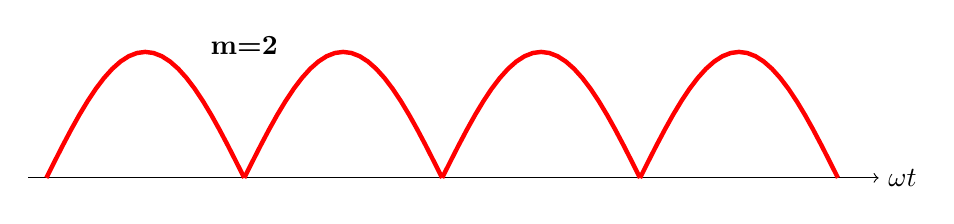
\begin{tikzpicture}
  \begin{scope}[xscale=0.8,yscale=1.6]
   \draw node[above] at (-pi/2,0.9)  {{\bf m=2}};
   \draw[thin, ->] (-5, 0) -- (8.5,0) node[right] {$\omega t$};
    % Vo and Io
    \foreach \qq [evaluate=\qq as \qqshft using \qq*pi] in {-1,...,2}
     {
      \begin{scope}[xshift=\qqshft cm,
          every path/.style={ultra thick, color=red}]
        %Vo
        \draw[domain=-pi/2:pi/2]
        plot (\x,{cos(\x r)})
        ;        
       \end{scope}
     }
\end{scope}
\end{tikzpicture}
\caption{m=2, E = 0.9}
\end{figure}

\begin{figure}[H]
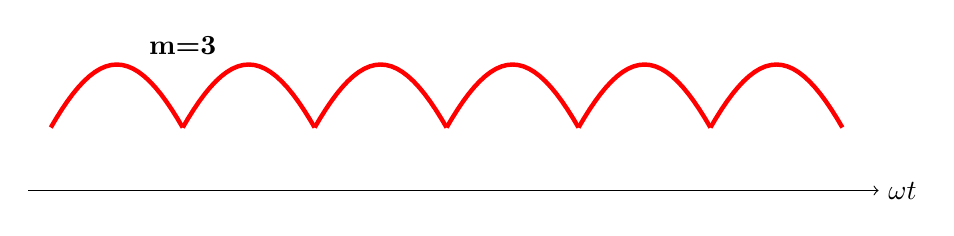
\begin{tikzpicture}
  \begin{scope}[xscale=0.8,yscale=1.6]
   \draw node[above] at (-pi/3,1)  {{\bf m=3}};
   \draw[thin, ->] (-3.5, 0) -- (10,0) node[right] {$\omega t$};
    % Vo and Io
    \foreach \qq [evaluate=\qq as \qqshft using \qq*2*pi/3] in {-1,...,4}
     {
      \begin{scope}[xshift=\qqshft cm,
          every path/.style={ultra thick, color=red}]
        %Vo
        \draw[domain=-pi/3:pi/3]
        plot (\x,{cos(\x r)});        
       \end{scope}
     }
\end{scope}
\end{tikzpicture}
\caption{m=3, E = 0.866}
\end{figure}


\begin{figure}[H]
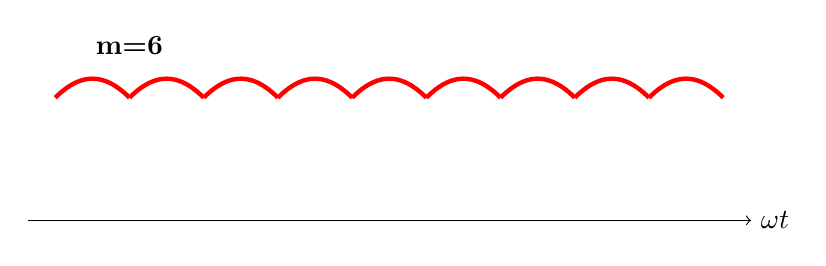
\begin{tikzpicture}
  \begin{scope}[xscale=0.9,yscale=1.8]
   \draw node[above] at (-pi/2,1.1)  {{\bf m=6}};
   \draw[thin, ->] (-3, 0) -- (7.2,0) node[right] {$\omega t$};
    % Vo and Io
    \foreach \qq [evaluate=\qq as \qqshft using \qq*pi/3] in {-2,...,6}
     {
      \begin{scope}[xshift=\qqshft cm,
          every path/.style={ultra thick, color=red}]
        %Vo
        \draw[domain=-pi/6:pi/6]
        plot (\x,{cos(\x r)})
        ;        
       \end{scope}
     }
\end{scope}
\end{tikzpicture}
\caption{m=6, E = }
\end{figure}

\begin{figure}[H]
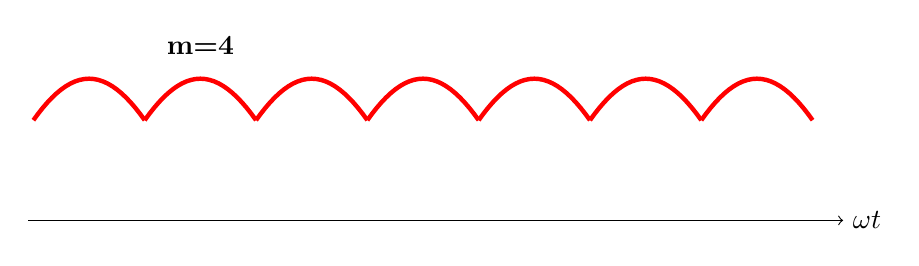
\begin{tikzpicture}
  \begin{scope}[xscale=0.9,yscale=1.8]
   \draw node[above] at (-pi/2,1.1)  {{\bf m=4}};
   \draw[thin, ->] (-4, 0) -- (7.5,0) node[right] {$\omega t$};
    % Vo and Io
    \foreach \qq [evaluate=\qq as \qqshft using \qq*pi/2] in {-2,...,4}
     {
      \begin{scope}[xshift=\qqshft cm,
          every path/.style={ultra thick, color=red}]
        %Vo
        \draw[domain=-pi/4:pi/4]
        plot (\x,{cos(\x r)})
        ;        
       \end{scope}
     }
\end{scope}
\end{tikzpicture}
\caption{m=4, ${\displaystyle E = \frac{\sqrt{2}}{2}}$}
\end{figure}

Вернулись к однополупериодной схеме

\begin{figure}[H]
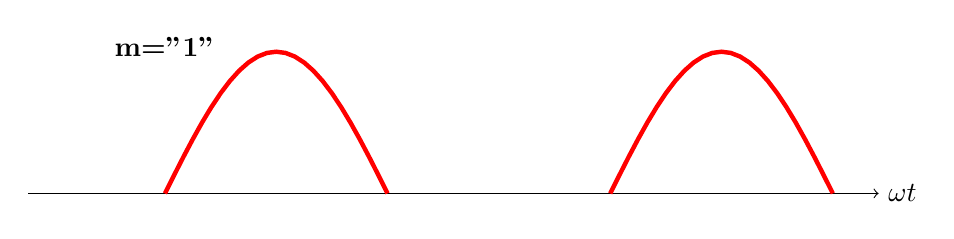
\begin{tikzpicture}
  \begin{scope}[xscale=0.9,yscale=1.8]
   \draw node[above] at (-pi/2,0.9)  {{\bf m=''1''}};
   \draw[thin, ->] (-3.5, 0) -- (8.5,0) node[right] {$\omega t$};
    % Vo and Io
    \foreach \qq [evaluate=\qq as \qqshft using \qq*pi] in {0,2}
     {
      \begin{scope}[xshift=\qqshft cm,
          every path/.style={ultra thick, color=red}]
        %Vo
        \draw[domain=-pi/2:pi/2]
        plot (\x,{cos(\x r)})
        ;        
       \end{scope}
     }
\end{scope}
\end{tikzpicture}
\caption{m=''1'', E = 0.45}
\end{figure}

Что осталось? Досчитать ${\scriptstyle} \Delta U_d$

$$
{\scriptstyle} \Delta U_d = \frac{2}{2\pi}\left\{
\int\limits_{-\frac{\pi}{m} + \alpha}^{\frac{\pi}{m} + \alpha} L_\phi \frac{d i_\phi}{dt} d\omega t +
\int\limits_{-\frac{\pi}{m} + \alpha}^{\frac{\pi}{m} + \alpha} ( i_\phi r_\phi + i_\phi R_d + U_0 + I_d R_\Phi)d\omega t
\right\} =
$$

$$
U_\phi = e_\phi - L_\phi \frac{\partial i_\phi}{\partial t} - i_R i_\phi
$$

1-й интеграл. смотрим на график $i$
$$
\int\limits_{\frac{\pi}{m} + \alpha \rightarrow {\textcyrillic{в момент включения самой фазы i}}}
^{\frac{\pi}{m} + \alpha \rightarrow {\textcyrillic{в момент включения следующей фазы}}}
\omega L_\phi \frac{di_\phi}{d(\omega t)} d\omega t
$$

$$
\frac{m}{2\pi}\left\{
\underbrace{\left. L_\phi i_\phi \right|_{-\frac{\pi}{m} + \alpha}}_
{
\begin{array}{c}
i_\pi = I_d\; {\textcyrillic{ когда фаза}} \\
{\textcyrillic{начала включатся}}
\end{array}
}
-
\underbrace{ L_\phi i_\phi \bigr|_{\frac{\pi}{m} + \alpha}}_
{
\begin{array}{c}
=0\;{\textcyrillic{ когда фаза}} \\
{\textcyrillic{включилась}}
\end{array}
}
\right\}
$$

Делаем допущение: $i_\phi$ -- меньше чем площадь прямоугольника (приближённо на всём промежутка равно $I_d$ )
$$
\int i_\phi (r_\phi + R_D) d\omega t + \frac{m}{2\pi}(U_0 + I_d R_\Phi)\int d\omega t =
$$
$$
= \frac{m}{2\pi} I_d X_\Phi +
\underbrace{\int i_phi (r_\phi + R_D) d\omega t}_{\textcyrillic{это возьмём приближённо}} +(U_0 + I_D R_\Phi)
=
$$


\begin{tikzpicture}
\begin{scope}
\draw (0.5,0) -- (3.5,0);
\draw (0.5,0) -- (1,1.5);
\draw (1,1.5) -- (3.5,1.5);
\draw (3.5,1.5); -- (3.5,0);
\draw[thin] (0.5, 0.2) -- (0.5, 2.3);
\draw[thin] (1, 1.6) -- (1, 2.3);
\draw[thin, ->] (0.1, 2.1) -- (0.5, 2.1);
\draw[thin, <-] (1, 2.1) -- (1.6, 2.1) node[left,below] {$\gamma$};
\draw[thin]  (3.6,1.5) -- (4.2,1.5);
\draw[thin]  (3.6,0) -- (4.2,0);
\draw[thin, <->] (4.1,0) -- (4.1,1.5);
\node[right] at (4.2, 0.75) {$I_d$};
\node[right] at (2, -0.75) {${\displaystyle \frac{m}{2\pi}}$};
\end{scope}
\end{tikzpicture}
Площадь трапеции равна ${\displaystyle I_d\left( 2\pi m - \frac{\gamma}{2}\right)}$ 

$$
= \frac{m}{2\pi}I_d \left( \frac{2\pi}{m} - \frac{\gamma}{2}\right)\left(r_\phi + R_D\right)
$$

$$
{\scriptstyle \Delta} U_d = \frac{m}{2\pi} I_d X_\Phi + U_0 + I_d R_\Phi +
\left(r_\phi + R_D\right) \left( 1 - \frac{\gamma m}{4 \pi}\right) I_d
$$

$$
U_d = E_{d0} Cos \alpha - {\scriptstyle \Delta} U_d
$$

\begin{equation}
U_d = E_{d} - U_0 - \frac{m}{2\pi} X_\Phi I_d - I_d \left\{
R_\Phi + \left(r_\phi + R_D\right) \left( 1 - \frac{\gamma m}{4 \pi}\right) 
\right\}
\end{equation}

Осталось определить, как $\gamma$ зависит от тока.
